\documentclass[10pt]{cv}

\begin{document}

\begin{minipage}[t]{0.82\textwidth}
  \vspace{-\baselineskip}
  \vspace{4ex}
  \begin{center}
  {\HUGE{MARC PLANELLES}}\\[2ex]

  \icon{faAt}{12}{\href{mailto:marc@planelles.dev}{marc@planelles.dev}}
  \icon{faGithub}{12}{\href{https://github.com/tmpbeing}{github.com/tmpbeing}}
  \icon{faGlobe}{12}{\href{https://planelles.dev}{planelles.dev}}\\[1ex]


  \icon{faMapMarker}{12}{Aix-en-Provence, France}
  \icon{faPhone}{12}{+33 6 81 80 41 37}\\[2ex]
  \LARGE{SOFTWARE DEVELOPER}
  \end{center}
\end{minipage}
\begin{minipage}[t]{0.18\textwidth}
  \vspace{-\baselineskip}
  \vspace{5mm}
  {
    \setlength{\fboxsep}{0pt}
    \setlength{\fboxrule}{2pt}
    \fbox{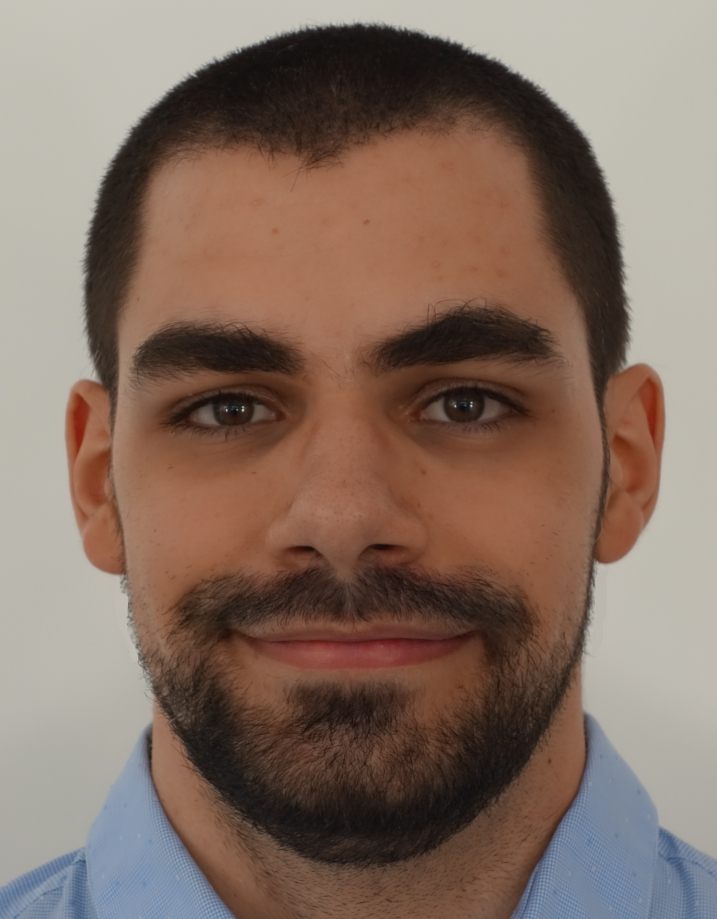
\includegraphics[width=\linewidth]{myface.jpg}}
  }
  % PHOTO SPACE %
  % \rule{2.8cm}{3.6cm}
\end{minipage}

%%%%%%%%%%%%%%
% EXPERIENCE %
%%%%%%%%%%%%%%

\vspace{2mm}
\cvsection{EXPERIENCE}

\begin{entrylist}
  \entry
    {5/2018 -- 11/2018}
    {Software Development Intern}
    {Tagsys}
    {\vspace{-1ex}
      \begin{itemize}
        \item Added monitoring to existing code
        \begin{itemize}
            \item[-] Wrote a statsD library with annotations
            \item[-] Inserted monitoring probes in existing code
            \item[-] Built infrastructure using InfluxDB/Telegraf/Granafa and Docker
          \end{itemize}
          \item Programmed controller to integrate new antenna into existing systems using its Rest API
          \item Programmed internal tool for database synchronization\\
      \end{itemize}
      \vspace{-1ex}
      \textit{Java / Spring / Hibernate / Docker /Telegraf / InfluxDB / Grafana}}
  \smallentry
    {2015 -- 2016}
    {Marketing Strategy and Community Management}
    {Warmcook}
  \smallentry
    {4/2014 -- 5/2014}
    {Marketing Assistant Intern}
    {Warmcook}
\end{entrylist}

%%%%%%%%%%%%%
% EDUCATION %
%%%%%%%%%%%%%

\vspace{-3mm}
\cvsection{EDUCATION}
\begin{entrylist}
  \smallentry
    {2017 -- ongoing}
    {42 Paris}
    {}
  \smallentry
    {2014 -- 2015}
    {1 Year in Master of IT Management}
    {Grenoble École de Management}
  \entry
    {2014}
    {Bachelor of Economics and Management}
    {Université Paul Cézanne}
    {With a specialization in international management}
  \smallentry
    {2010}
    {High School Diploma}
    {Lycée Paul Cézanne}
\end{entrylist}

\vspace{-2mm}

%%%%%%%%%%
% SKILLS %
%%%%%%%%%%

\begin{minipage}[t]{0.49\textwidth}
\cvsection{SKILLS}
\textbf{Working knowledge:}\\[0.5ex]
C, Java (Spring, Hibernate), Rust\\[0.5ex]
Git, Docker, Emacs/Vim, IDEA, GNU/Linux\\[1.2ex]
\textbf{Basic knowledge:}\\[0.5ex]
C++, Python, Common Lisp, HTML, CSS, Latex
\end{minipage}
\hfill
%
%%%%%%%%%%%%%%
% SELF-STUDY %
%%%%%%%%%%%%%%
%
\begin{minipage}[t]{0.49\textwidth}
\cvsection{SELF-STUDY}
\textbf{C:} The C Programming Language (K\&R), C Programming: A Modern Approach (K.N. King)\\[1.2ex]
\textbf{General:} Clean Code (R. Martin)\\[1.2ex]
\textbf{Java:} Head First Java (K. Serria and B. Bates), Effective Java (Joshua Bloch)\\[1.2ex]
\textbf{Lisp:} The Land of Lisp (C. Barski)
\end{minipage}

%%%%%%%%%%%%%
% LANGUAGES %
%%%%%%%%%%%%%

\begin{minipage}[t]{0.49\textwidth}
\cvsection{LANGUAGES}
\textbf{French:} native\\[1.5ex]
\textbf{English:} fluent/C2 level
\end{minipage}
\hfill
%
%%%%%%%%%%%%%
% INTERESTS %
%%%%%%%%%%%%%
%
\begin{minipage}[t]{0.49\textwidth}
\cvsection{INTERESTS}
Volunteered for Students for Liberty Aix-Marseille (2012 -- 2013)\\[0.5ex]
Reading fantasy, SF and non-fiction\\[0.5ex]
Synthesizers\\[0.5ex]
Emacs\\[0.5ex]
GNU/Linux ricing


\end{minipage}
\end{document}

% %%% Local Variables:
% %%% mode: latex
% %%% TeX-master: t
% %%% End:
